\documentclass{extarticle}

\usepackage{graphicx}
\usepackage{enumerate}
\usepackage{amsthm}
\usepackage{amsmath}

\begin{document}

\begin{titlepage}
\title{Design Document for Kairos Constraint-Based Scheduling Software System}
\author{Tyler Chapman, Nate Crandall, Vinh Dang, Vince Oveson, Tony Tuttle}
% INSERT TEAM LOGO
\maketitle
\thispagestyle{empty}
\end{titlepage}

\tableofcontents

\newpage

\section{Executive Summary} % ONE PAGE

\subsection{Overview}
% DESCRIBE THE FINAL GOAL OF THE PROJECT
%   - what the project will do
The final goal of the project is to provide a highly customizable, open-source, web-based scheduling tool available
to solve a wide range of scheduling problems.  Our software system will be accessible through a public
website where users may build, modify, and maintain their solutions.  The system will be capable of solving various
types of scheduling problems for various types of user needs.

%   - what need it will address
Scheduling problems are ubiquitous.  Individuals, teams, organizations, and larger entities such as companies all
must solve scheduling problems of various levels of complexity.  Our tool aims to address the needs of such a wide
base of potential users.

\subsection{Features and Components}
% LIST KEY FEATURES AND COMPONENTS
%   - schedule solver
%   - web-based (open to all users)
%   - customizable
%   - well-written API
%   - thoughtful visualization component
At its core, Kairos will be a web-based schedule solver; it will accept parameters from the user, specifying the
details of their particular scheduling problem.  The tool will analyze the input and algorithmically determine a
schedule that will meet all of the supplied parameters.  If meeting all of the constraints is not possible, it will
prioritize based on weights and determine what compromises to make in the schedule.

Since the tool will be web-based, it will be open to any and all potential users.  This will further encourage a
wide breadth of users.

By keeping the core schedule solver as general as possible, we intend to make the tool as customizable as possible.
We want users to be have access to the powerful core components while maintaining sufficient flexibility to fit the
solution to their specific needs.

Part of this customizability will come from working hard to make the API as clear and thorough as possible.  A
great piece of software may lose potential users if it is not clear to users how best to leverage the software.  We
intend to encourage a large user base by putting a lot of emphasis on creating a strong API.

Likewise, a great piece of software that lacks intuitiveness or a pleasing user experience will alienate users.
We will put a great deal of thought and planning into determining how best to use visualization tools to represent
our data.  Since scheduling is a complex problem that produces data that will need to be viewed from several angles,
this is a difficult problem in itself.  By making visualization a priority we hope to attract users as opposed to
driving them away.

\subsection{Justification}
% EXPLAIN WHY THE PROJECT IS INTERESTING AND WORTHWHILE
%   - why a completed project will be beneficial
Making this tool available to the public will potentially save individuals a great deal of time, may provide
organizations better scheduling solutions than they currently have, and could potentially save a great deal
of money for businesses and other organizations.  At the very least it is our hope that we will make life a little
easier for as many users as possible.

\section{Background}

\subsection{Overview} % ONE TO THREE PAGES
%   - why our project is needed
Scheduling is a problem that is faced in some way by all individuals as well as groups, teams, and other
organizations of all sizes.  
%   - what problems it solves
%   - who will use it
\subsubsection{Similar Ideas}
% list, describe other software systems that do what ours will do
% explain why our idea is different and/or better
Aurora is an existing scheduling system. However, from our understanding, Aurora, as well as many other scheduling solutions such as Microsoft Project, Primavera, or Open Workbench, focus on project scheduling with multiple task sequences, or critical paths, in which previous tasks need to be completed before the next one can begin.

Figure \ref{fig:aurora}, taken from Aurora's website, is an example of its usage. In this figure, activities 1, 5, and 6 (the ones in red) must be executed sequentially in that order, hence the name critical path. Also noted that all the activities in the figure last more than or equal to one day. That's how a usual project task is, it either lasts for a couple of days, or requires, for instance, 20 hours/week to complete (for Open Workbench). Because of this, these systems are not really suitable for scheduling meetings or events that need ``small" specific time slots with no actual ``critical path" most of the time. They may be used and/or tweaked to do this, but the experience probably won't be good since that's not what the systems are designed for.

This is where our system shines. We want to create a system that can apply resource-constraint into meeting/event scheduling, just as how it's been done with project scheduling. The system will support fine-grained control over possible time blocks. It will allow users to specify available resources (human, room, capacity, and so on), and constraints via a uniform, easy-to-understand API. Not only that, the users will also be able to edit the suggested schedule easily to better suit their need and preference.

\begin{figure}[H]
\centering
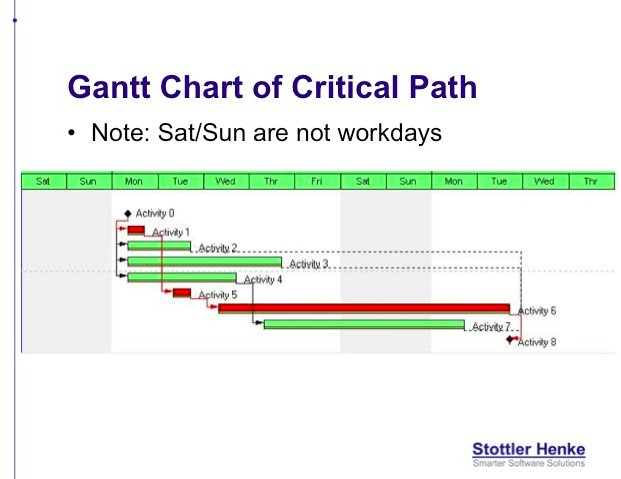
\includegraphics[width=90mm]{aurora.jpg}
\caption{Aurora scheduling example}
\label{fig:aurora}
\end{figure}


\subsection{Required Technology}
% list, describe software technologies that you will:
%   - need to implement
%   - need to utilize

% assets and engines
%   - how much will be built from scratch
%   - what resources, assets (and from where) will be leveraged

\subsection{Software/Hardware Requirements}
% what hardware, software we will need to successfully installed in order to use our software


\end{document}
